\mysubsection{Du modèle client/serveur aux applications "web"}

\ifbook{
  \mysubsubsection{Bref histoire du client léger}
  \paragraph{} Avec l'apparition des réseaux informatiques, apportés par des technologies telles que
  TCP/IP sur laquelle s'est construit le désormais célèbre protocole HTTP, il est rapidement apparu
  très intéressant de pouvoir répartir le traitement sur plusieurs machines.

  \paragraph{} En effet, au début de l'informatique, les machines puissantes coûtaient relativement
  cher, et avaient des capacités de calcul permettant d'effectuer des calculs complexes et de
  répondre aux besoins de nombreux utilisateurs. Ainsi est né le modèle client/serveur, où
  l'utilisateur, à l'aide d'un terminal - une machine peu puissante et peu coûteuse de comme le minitel
   - se connecte à une machine lui servant des données et exécutant les traitements demandés - un serveur. 
  Le terminal se contentant, dans ce modèle, d'afficher le résultat.

  \begin{figure}[h]
    \begin{center}
      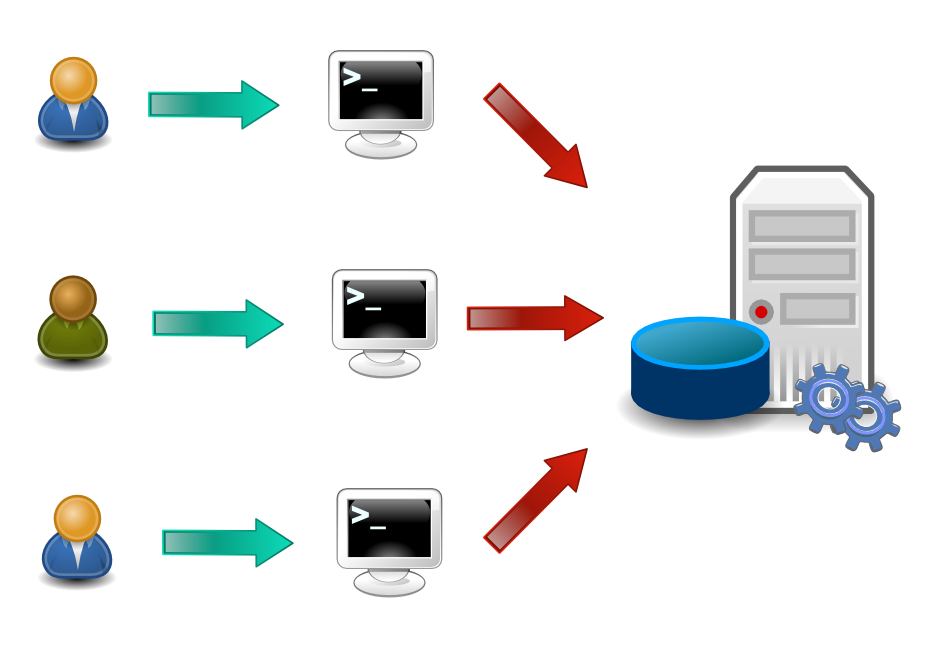
\includegraphics[scale=0.3]{img/mainframe-terminals.png}
      \caption{Terminaux et mainframe}
      \label{mainframe}
    \end{center}
  \end{figure}
}

\ifslide{
  \begin{frame}{Mainframe et terminaux}
    \begin{center}
      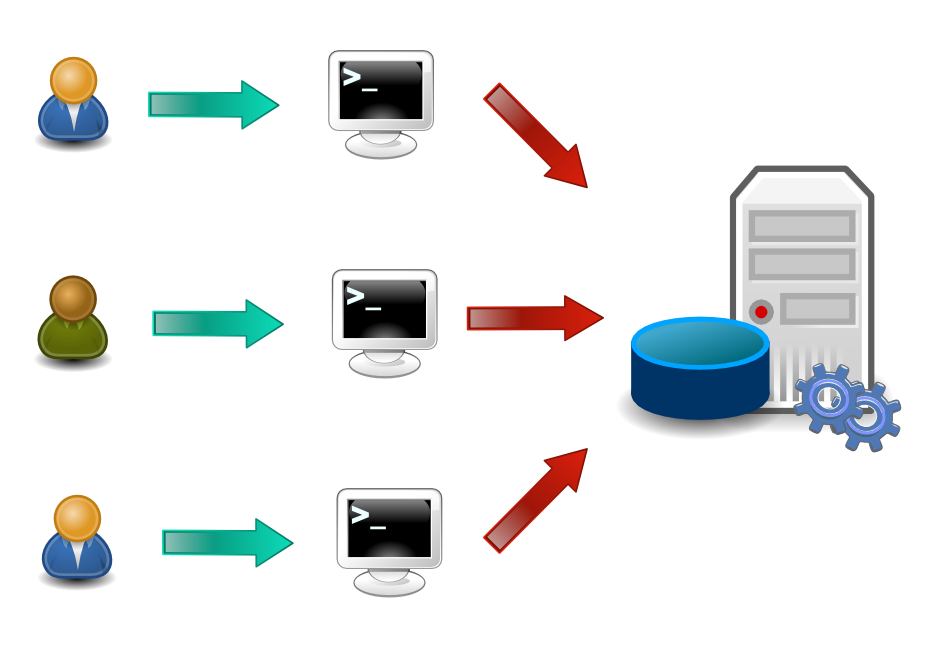
\includegraphics[scale=0.3]{img/mainframe-terminals.png}
    \end{center}
  \end{frame}
}

\ifbook{

  \paragraph{} Avant d'aller plus loin, on peut noter avec intérêt que ce modèle n'est en fin de
  compte pas très différent de celui des débuts d'internet. En effet, à leurs débuts, les
  navigateurs "web" (Mozaic, Netscape, puis Internet Explorer) se contentaient simplement d'afficher le
  contenu des pages HTML qu'on leur servait. Nous y reviendrons par la suite...

  \mysubsubsection{La naissance du client "lourd"}

  \paragraph{} Ce premier modèle client/serveur se construisait donc sur deux logiciels distincts,
  une première partie s'exécutant sur le terminal de l'utilisateur, le \textbf{client léger}, et une
  seconde partie, plus élaborée et embarquant la \textbf{logique métier} de l'application, le
  \textbf{serveur}.

  \paragraph{Remarque} \textit{L'usage a malheureusement imposé depuis longtemps l'utilisation du même
  terme, \textit{serveur} pour désigner deux entités conceptuellement similaire, mais concrètement
  différentes. Ce terme peut en effet indiquer une machine physique, un ordinateur, relié à un
  réseau informatique et utilisé, à distance, par des utilisateurs, mais aussi le logiciel s'exécutant
  sur ce même type d'ordinateur et fournissant un service applicatif à ces mêmes utilisateurs.}

  \paragraph{} \textit{La différence est relativement aisée à saisir, mais elle peut tout de même
  prêter à confusion. Si dans le cas de la partie précédente nous évoquions le concept de machine
  physique, dans cette section, nous parlons très clairement de \textbf{serveur logiciel}.}

  \paragraph{} Alors que la puissance à la disposition des terminaux augmentait, et que, dans les
  faits, ceux-ci devinrent des ordinateurs graphiques à usage personnel ("\textit{Personal Computer
  (PC)}"), il apparut rapidement très pertinent d'en profiter pour offrir des clients plus puissants,
  capable d'effectuer des traitements par eux-mêmes, et donc offrir des fonctionnalités
  supplémentaires à leur utilisateurs.

  \paragraph{} Ainsi le mouvement de balancier, qui avait pour but de placer le maximum de logique
  applicative et de traitement du côté du \textit{serveur}, s'est inversé et les logiciels clients
  devinrent à leur tour de plus en plus complexe, au point qu'on les qualifia de \textbf{clients
  lourds}.

  \begin{figure}[h]
    \begin{center}
      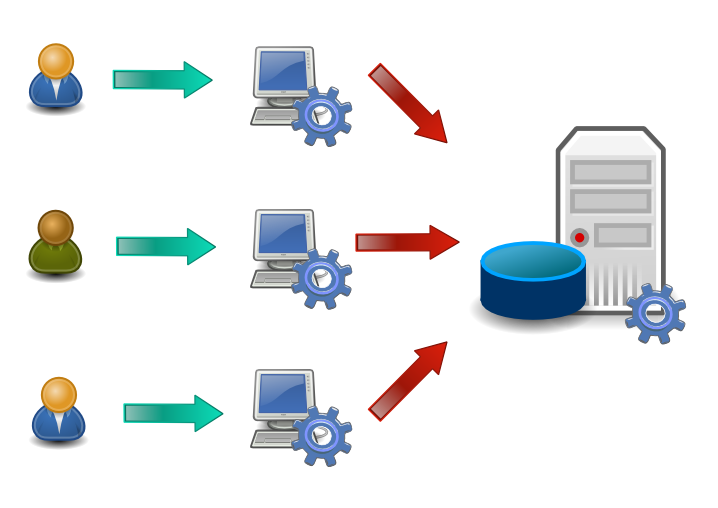
\includegraphics[scale=0.3]{img/fat-clients.png}
      \caption{L'arrivée du PC et des clients lourds}
      \label{fat-clients}
    \end{center}
  \end{figure}

  \mysubsubsection{Les limites du modèle}

  \paragraph{} Si cette nouvelle déclinaison du modèle aboutit clairement à une meilleure productivité
  des utilisateurs, du moins dans la plupart des cas, elle posa aussi rapidement des problématiques
  complexes en terme de maintenance. En effet, pour pouvoir faire évoluer le logiciel, il faut
  désormais modifier à la fois le client et à la fois le serveur, et assurer leur redéploiement
  synchrone. On se retrouva vite malheureusement dans des situations difficiles à gérer, où de
  multiples versions d'une même application clientes étaient déployées et devaient cohabiter avec des
  versions différentes de leurs serveurs...
}

\ifslide {
  \begin{frame}{Le modèle client/serveur}
    \begin{center}
      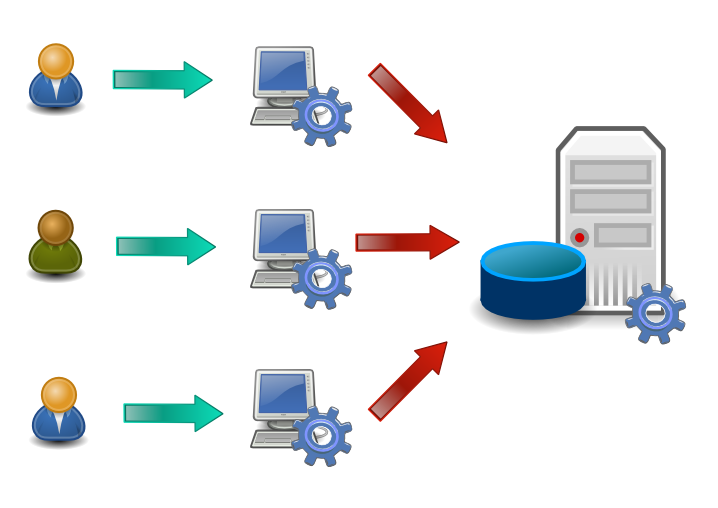
\includegraphics[scale=0.3]{img/fat-clients.png}
    \end{center}
  \end{frame}
}

\ifbook{
  \mysubsubsection{La Persistance des données: du fichier à la base de données}
  % fichier et répertoires
  \paragraph{} Avant de voir comment les technologies de type client/serveur ont évolué pour
  circonvenir les problématiques apparues avec l'émergence du client lourd, intéressons-nous un instant
  non plus au logiciel, mais à ses données, et surtout à leur persistance.

  \paragraph{} Comme évoqué plus haut, un ordinateur travaille avec des données en mémoire qui
  sont donc par essence, \textbf{volatiles}. En effet, lors de l'interruption de l'alimentation de la
  mémoire, les données qu'elle contient sont purement et simplement perdues. Les données n'étant,
  dans la plupart des applications, que rarement dispensables, il a été impératif de trouver des
  mécanismes pour assurer leur \textbf{persistance}.

  \paragraph{} L'unité atomatique de cette persistance est le \textbf{fichier}. Cette abstraction
  permet de sauvegarder sur une unité de stockage (en langage vernaculaire, un "disque dur") un ensemble 
  d'information de manière séquentielle. On peut retrouver les informations stockées à l'aide du nom 
  du fichier.

  \paragraph{} En fait, on peut aisément comparer un fichier à une simple feuille, sur laquelle on
  écrit les données que l'on souhaite voir persister, un peu de la même manière dont on écrit sur une
  feuille sa liste de courses, pour justement, ne pas l'oublier.

  \paragraph{} Pour permettre de trier et de ranger ses fichiers, dans la prolongation de l'image
  choisie pour les fichiers, des fichiers spéciaux, les \textbf{répertoires} ont été conçu pour
  permettre de ranger aisément et hiérarchiquement ces fichiers.

  \paragraph{} Malheureusement, la manière séquentielle d'organiser les informations d'un fichier
  se révéla contraignante. En effet, alors que les applications se complexifiaient, et qu'une donnée
  fit référence à une autre, puis à une autre, la nature \textbf{relationnelle} devint évidente et
  imposa un changement de stratégie dans l'approche de leur persistance.

  \paragraph{} En outre, les données nécessitent bien souvent d'être partagées entre plusieurs
  applications, et il est fort complexe de partager un fichier de données entre plusieurs
  applications. Comment gérer les accès concurrents ? Comment assurer la cohérence des données qui
  ont été persistées ?
  % base de donnée
  \paragraph{} Pour palier à ces nombreux problèmes et surtout clairement séparer les données des
  applicatifs, les premières bases de données relationnelles firent leur apparition. En plus de
  permettre de stocker les données hors des applications et de les partager, elles permirent, peu à
  peu, d'établir un langage standard pour interagir avec elles, le SQL (\textit{Standard Query
  Language}).
}

\demoframe{Le SQL}{
  \begin{center}
    Une rapide démonstration du langage SQL....
  \end{center}
}

\ifbook{
  \mysubsubsection{Architecture n-tiers}
    \paragraph{} Si nous résumons les différents éléments évoqués jusqu'à maintenant sous forme de
    la figure \ref{n-tiers} (page \pageref{n-tiers}), on constate que désormais notre application,
    qui au départ s'exécutait sur une seule machine, reliée par un terminal très primaire, est
    désormais réellement éclatée entre plusieurs composants, ou \textbf{tiers}.

    \paragraph{} Ainsi, de l'architecture client/serveur, composé de deux tiers, on est arrivé à une
    architecture 3 tiers, où la base de données vint s'ajouter, en tant que troisième tiers. Mais en
    fait, la séparation des fonctions sur différentes instances physiques a continué, et
    aujourd'hui on parle plus en plus souvent d'architecture \textbf{n-tiers}.

    \begin{figure}[h]
      \begin{center}
        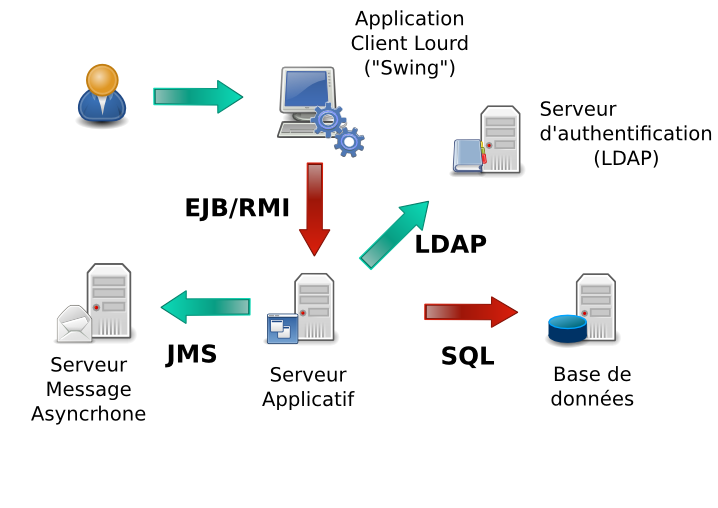
\includegraphics[scale=0.3]{img/n-tiers.png}
        \caption{Exemple d'architecture n-tiers}
        \label{n-tiers}
      \end{center}
    \end{figure}
}

\ifslide{
  \begin{frame}{Architecture n-tiers}
    \begin{center}
      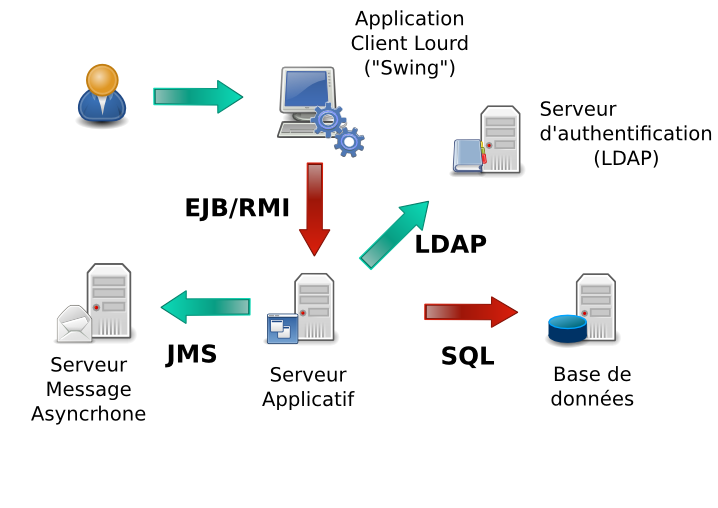
\includegraphics[scale=0.35]{img/n-tiers.png}
    \end{center}
  \end{frame}
}
